

\setcounter{section}{1}
\section{System Overview}
\bigskip

The Akriveia Beacon indoor locating rescue system combines hardware, electrical, and software systems to detect and locate multiple occupants within a building during an emergency disaster situation. Each individual component of the system is developed separately in the PoC (Proof of Concept) phase; then partially integrated in the Prototype phase and fully integrated in the Final Product phase. 

\bigskip
A high-level system overview presents three Locator Beacons, an ID tag, a data processing unit, and a graphical user interface (Figure \ref{sys_arch}). Using ultra-wideband (3.5-6.5 GHz) wireless communication the Locator Beacons transmit signals to the ID tag to acquire a response. When the response returns back to the Beacon a time of flight measurement is acquired. The Time-of-Flight principle (ToF) is a method for measuring the distance between a sensor and an object, based on the time difference between the emission of a signal and its return to the sensor, after being reflected by an object. \cite{R2-0}. The ToF data will be forwarded to the portable data processing unit via a closed Wi-Fi network with UDP.  Then the processing unit will calculate the distance and coordinates of the ID tags using trilateration algorithm. Afterwards, the coordinates results are displayed on a GUI for operators.

\medskip
\begin{figure}[H]
\centering
    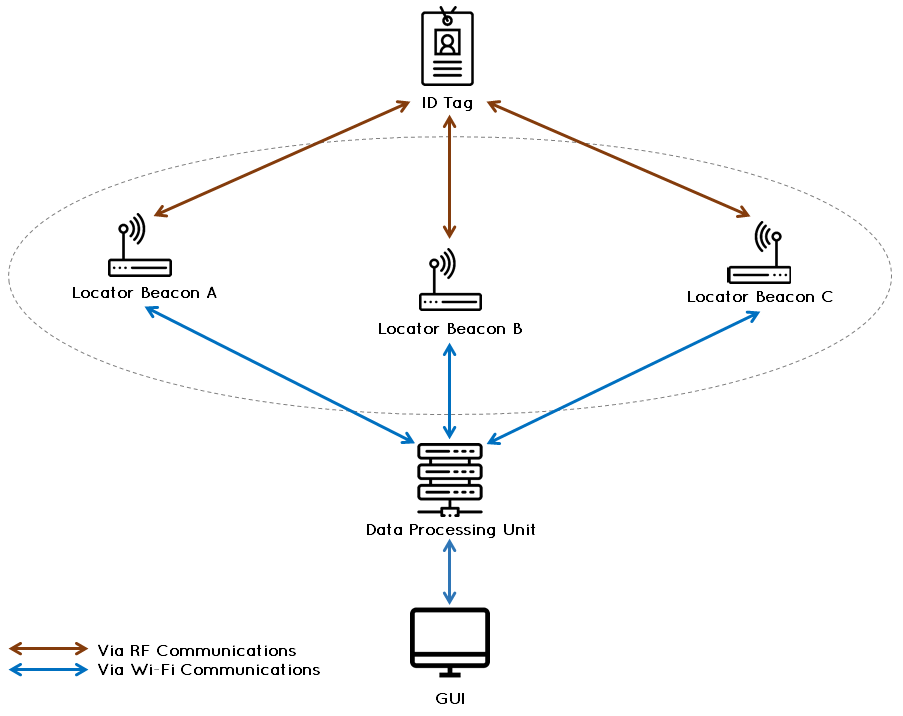
\includegraphics[scale=0.65]{./images/00_sys_arch.png}
    \caption{High Level System Layout}
    \label{sys_arch}
\end{figure}



\pagebreak
\subsection{Proof of Concept}
\medskip
The Proof of concept phase demonstrates the feasibility and functionality of an indoor location determination system. The PoC system will evaluate how effect a trilateration method is to determine the distance and location of a mobile  ID tag in two dimensional space as well as to establish an initial development system. Similar to the system block diagram shown in figure \ref{poc}.

\bigskip
ESP32 micro-controllers are used as the main hardware components of the Beacon and ID Tags. The ESP32 is an off the shelf, low-cost, low-power system on a chip micro-controllers with integrated Wi-Fi and dual-mode Bluetooth. Received Signal Strength Indicator (RSSI) from Bluetooth Low Energy (BLE) modules are used to estimate distance between each beacon and ID tag. Each beacon determines the MAC address and a RSSI measurement from the advertising ID Tag. The data is forwarded to the data processing unit - Raspberry Pi, via USB serial communication. The RSSI is then used to estimate distance between each ID Tag and the associating Beacon and the results are output to a simple UI. 

\medskip
\begin{figure}[H]
\centering
    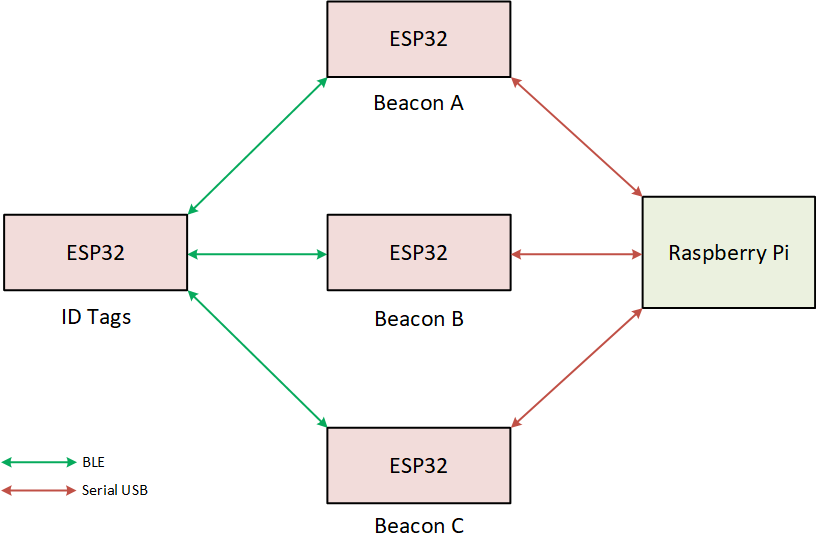
\includegraphics[width=\linewidth]{./images/01_poc.png}
    \caption{PoC System Block Diagram}
    \label{poc}
\end{figure}



\pagebreak
\subsection{Prototype}
\medskip
In the Prototype development phase the transceivers will be incorporated with Decawave DWM1000 UWB modules. The DWM1000 UWB uses radio frequencies in the range of 3.5 to 6.5 GHz; this would significantly reduce issues of signal interference or multipath propagation which would occur by using RSSI with BLE. The DWM1000 will be incorporated as the transceiver with the ESP32 as the main MCU as shown in figure \ref{prototype} below. RF data communication functions will be established between four UWB modules with one as the ID Tag and three as the Locator Beacons to demonstrate distance estimation with DWM1000 UWB modules. This will be achieved by using signal fingerprinting to determine transmitter properties such as ToF and unique Tag identifier. Furthermore, trilateration algorithms will be implemented on data processing unit to determine near real time location and coordinates of ID Tags. Initial Implementation of software stack on data processing unit and development of GUI will occur during this phase as well.

\medskip
\begin{figure}[H]
\centering
    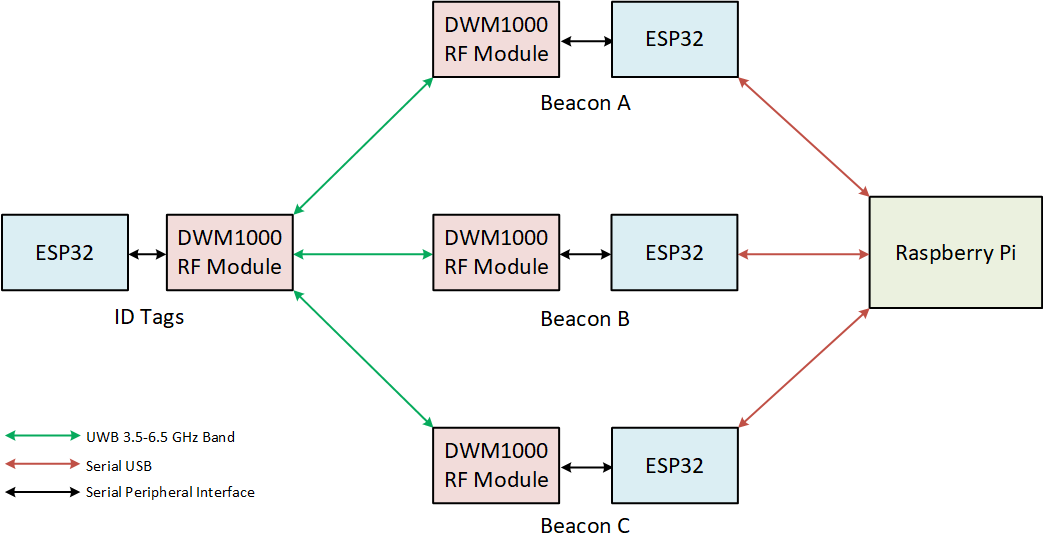
\includegraphics[width=\linewidth]{./images/02_prototype.png}
    \caption{Prototype System Block Diagram}
    \label{prototype}
\end{figure}


\pagebreak
\subsection{Final Product}
\medskip
The final product will demonstrate the fully functional indoor rescue system that detects the location of the ID tags and displays it accordingly on a GUI. Here the addition of ESP32’s Wi-Fi modules can be seen (Figure \ref{final}), as the Beacon will communicate via Wi-Fi communication with the data processing unit. The Wi-Fi network will be a closed network meaning that the network is only share between beacons and the data processing unit to ensure security, reliability and stability. Furthermore, implementation of RF harvesting circuit for ID Tag device charging during deep sleep mode will occur during this stage. All the components of the systems will be fully integrated as a close-to-production product. Component circuits and PCB footprint will be minimized and proper casing will be made to house all electronics. The data processing unit will provide the user with a full GUI to interact with the system along with the fully implemented features such as importable blueprints and multi-floor tracking.

\medskip
\begin{figure}[H]
\centering
    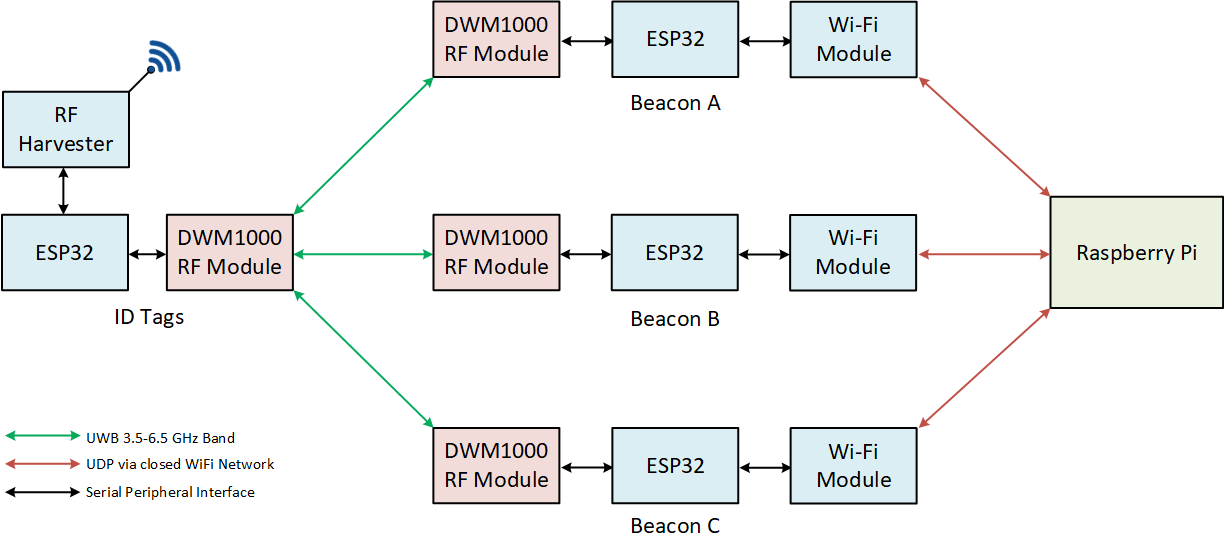
\includegraphics[width=\linewidth]{./images/03_final.png}
    \caption{Final System Block Diagram}
    \label{final}
\end{figure}




\pagebreak
\subsection{Ultra-Wideband Radio Technology}
\medskip



\pagebreak
\subsection{Trilateration Methods}


